\chapter{编队控制器设计}
\label{chap:controller_design}
第\ref{chap:formation_dynamic_equ}章中介绍了无人机双机编队的动力学模型,并将无人机运动分为铅垂平面以及水平平面;方程组\ref{fol_motion_eauation1}水平平面的直接输入量为$\Psi$的期望值,铅垂平面的
直接输入量为$\theta$和$V$的期望值。整体的控制逻辑框图如下图所示:
\begin{figure}[H]
    \centering
    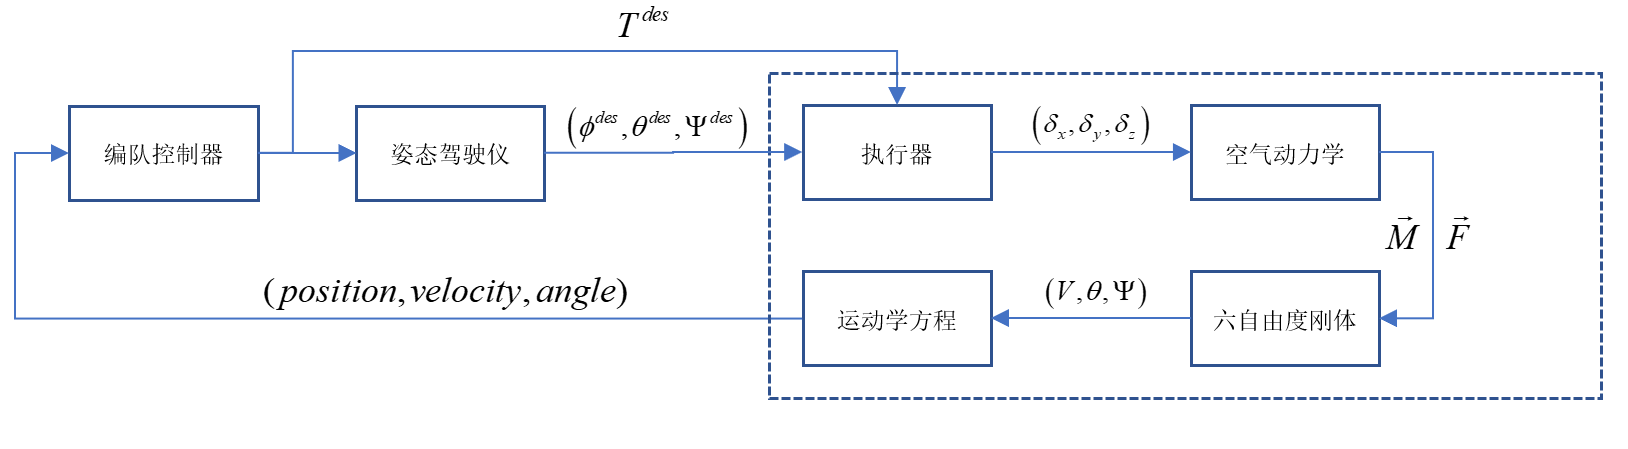
\includegraphics[width=0.85\textwidth]{figures/c3/c3-overview_controller.png}
    \caption{控制逻辑框图}\label{fig:c3-overview_controller}
\end{figure}
编队控制器的输入为定义的误差量,输出为无人机自动驾驶仪的内环输入值,即期望推力$T^{des}$,期望姿态$\Phi^{des},\theta^{des}$,偏航期望值$\Psi^{des}$将由内环姿态
自动驾驶仪按照协调转弯条件计算得到。本章的剩余部分将分别设计铅垂平面以及水平平面的控制器。
%TODO:此处的分配方式有些问题,考虑机体x和y;初步完成对于两个方向的分别
\section{水平平面编队控制器设计}
\subsection{误差定义}
导航的本质是控制地速的方向,实现手段是产生垂直于速度方向的法向加速度$a_{y_b}^{des}$;在无人机之中,多采用协调转弯(BTT)方式产生法向加速度。在导弹的制导规律之中,制导的最终目标是与期望的
点相交,而编队控制器的最终目标为:
\begin{enumerate}
    \item 从机速度方向与领机的速度方向一致。
    \item 从机的速度大小与领机的速度大小一致。
    \item 从机的位置与从机的期望位置一致。
\end{enumerate}
此处产生三种误差类型,这三类误差均投影在从机机体坐标系$O_bx_by_bz_b$之中,便于之后产生控制量:
\begin{enumerate}
    \item 领机与从机2维速度方向误差$\eta$。%TODO:记得改一下图,与之对应
    \item 领机与从机速度(地速$V_g$)大小误差$|V_g|^{err}$。
    \item 领机与从机3维位置误差$(P_{x_b}^{err},P_{y_b}^{err},P_{z_b}^{err})$
\end{enumerate}
因而此处水平平面的编队控制器的控制的任务是消除水平平面内的位置误差、速度大小以及速度方向误差,前两者在机体系$O_bx_b$轴的分量需通过期望速度大小${|V|}^{des}$消除;前两者在机体系$O_by_b$轴
的分量,以及速度方向误差须通过期望法向加速度$a_{Y_b}^{des}$消除。值得注意的是:实际上此处的速度方向误差代表了机体系内的两分量之比值,实际上与角度误差代表同一误差,但是由于机体系$O_bx_b$轴
的期望速度时刻变化,而所需的速度方向须按照领机速度方向一致,因而要控制速度的方向,而不是单纯的$O_bx_b$轴的速度分量。
\subsection{机体系x轴方向控制器}
机体系$O_bx_b$轴方向的控制器的输入为速度大小误差以及位置误差沿本轴分量的混合,控制器选用增量式离散$PID$控制器,最终的控制量的输出为期望速度大小${|V|}^{des}$。控制器的表达式为:
\begin{equation}
    \left\{
    \begin{array}{l}
        |V_g|^{err}(k)=|V_g^{l}|(k)-|V_g^{f}|(k)\\
        P_{x_b}^{err}(k)=P_{x_g}^{des}(k)-P_{x_g}^{f}(k)\\
        e_{x_b}(k)=K_V|V_g|^{err}(k)+K_{Px}P_{x_b}^{err}(k)\\
        \begin{aligned}
        \Delta{|V|}^{des}(k)=&K_{p}^{xmix}[e_{x_b}(k)-e_{x_b}(k-1)]+K_{i}^{xmix}e_{x_b}(k)+\\
        &K_{d}^{xmix}[e_{x_b}(k)-2e_{x_b}(k-1)+e_{x_b}(k-2)]
        \end{aligned}
        \\
        {|V|}^{des}(k)=\Delta{|V|}^{des}(k)+{|V|}^{des}(k-1)
    \end{array}
    \right .
    \label{xb_vel_gen_equ}
\end{equation}
其中,前3式定义了混合误差形式,实际为速度误差与位置误差的线性叠加。后2式表示了最终的期望速度大小的产生。$K_V,K_P$为误差线性混合常数。$K_{p}^{xmix},K_{i}^{xmix},K_{d}^{xmix}$为增量式离散
$PID$控制器参数。

此处产生的期望速度大小,并不能直接为内环姿态驾驶仪所响应,需要经过铅垂平面控制器的计算,位置误差$P_{z_b}^{err}$共同产生期望油门以及期望俯仰角。
\subsection{机体系y轴方向控制器}
机体系$O_by_b$轴方向的控制器的输入为速度方向误差$\eta$以及位置误差的混合,类似于机体系$O_bx_b$轴方向的控制器,控制器也选用增量式离散$PID$控制器,最终的输出为无人机滚转角期望值。
由图\ref{fig:c02-2d_level_motion}可得到:
\begin{equation}
    \eta^f=\Psi^l-\Psi^f
    \label{yaw_error}
\end{equation}
上式得到的是无人机速度方向的角度误差;因而最终的误差形式为:

再考虑如图所示的无人机二维平面转弯运动:
\begin{figure}[H]
    \centering
    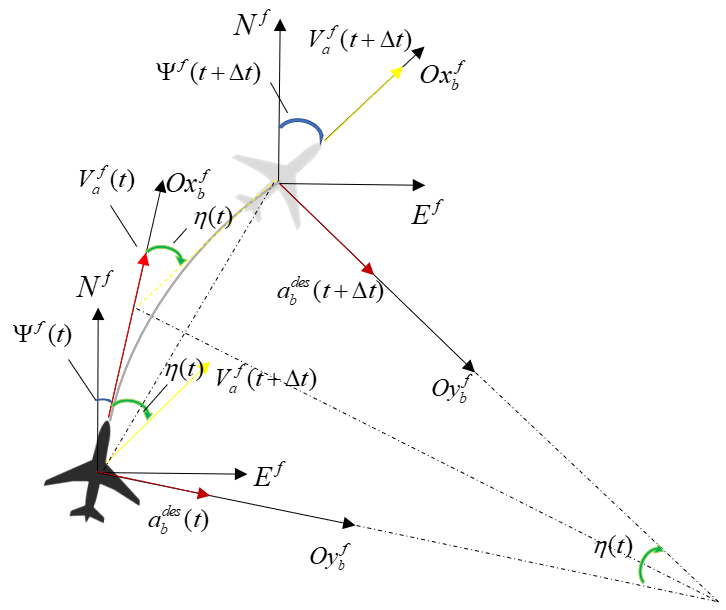
\includegraphics[width=0.5\textwidth]{figures/c3/c3-BTT.png}
    \caption{无人机二维平面转弯运动}\label{fig:c3-BTT}
\end{figure}
由于飞机速度的动力学惯性很大,在微分时间$\Delta t$时间内,速度的变化量可以忽略不计;在此时间内的偏航角增量为$\Delta\eta$,按照图中的几何关系,不难得到:
\begin{equation}
    a_{x_b}=V_g\dot{\eta}
    \label{btt_dot}
\end{equation}
上式即无人机期望偏航角速度与期望法向加速度关系。类似于上一节,定义混合误差为角度误差以及距离误差的线型混合。
再利用上一小节提出的增量式离散$PID$控制器,再综合式\ref{yaw_error},可得混合误差到期望法向加速度的表达式为:
\begin{equation}
    \left\{
        \begin{array}{l}
            \eta^f(k)=\Psi^l(k)-\Psi^f(k)\\
            P_{y_b}^{err}(k)=P_{y_g}^{des}(k)-P_{y_g}^{f}(k)\\
            e_{y_b}(k)=K_{\eta}\eta^f(k)+K_{Py}P_{y_b}^{err}(k)\\
                \begin{aligned}
                \Delta\dot{\Psi}^{des}(k)=&K_{p}^{ymix}[e_{y_b}(k)-e_{y_b}(k-1)]+K_{i}^{ymix}e_{y_b}(k)+\\
                &K_{d}^{ymix}[e_{y_b}(k)-2e_{y_b}(k-1)+e_{y_b}(k-2)]
                \end{aligned}\\
            \dot{\Psi}^{des}(k)=\Delta\dot{\Psi}^{des}(k)+\dot{\Psi}^{des}(k-1)\\
            \dot{\eta}^{des}(k)=-\dot{\Psi}^{des}(k)\\
            a_{y_b}^{des}(k)=-V_g^{f}(k)\dot{\eta}^{des}(k)
    \end{array}
\right .
    \label{angle_controller}
\end{equation}
上式得到的是期望法向加速度,再利用协调转弯(BTT)条件,将期望法向加速度,转化为期望滚转角:
\begin{equation}
    \tan\Phi^{des}(k)=\frac{a_{y_b}^{des}(k)}{g}
    \label{btt_a2roll}
\end{equation}
其中,$g$为当地重力加速度常量。至此,水平平面面内可计算得到无人机的期望滚转角$\Phi^{des}$以及期望速度大小$|V|^{des}$
\section{铅垂平面编队控制器设计}
铅垂平面编队控制器的输入为期望速度大小$|V|^{des}$以及期望高度(实际代表了高度误差$P_{z_b}^{err}$),输出为期望俯仰角$\theta^{des}$以及期望推力$T^{des}$。控制器选用基于能量的总能量控制法
(total energy control system,$TECS$)。固定翼无人机的速度控制和高度控制是耦合的,即单独控制高度或速度时,另一个未被控制量将会发生变化:
下面通过飞机飞行动力学纵向运动方程简单说明:
方程组\ref{fol_motion_eauation1}的第三式说明:飞机高度方向的变化率与地速大以及俯仰角大小有关,且为正相关。
飞机纵向运动质心运动的动力学方程抄录如下:
\begin{equation}
    \left\{
    \begin{aligned}
    &m \frac{\mathrm{d} V}{\mathrm{d} t}=T \cos (\alpha+\varphi) \cos \beta-D-m g \sin \gamma\\
    &m V \cos \gamma \frac{\mathrm{d} \chi}{\mathrm{d} t}=T[\sin (\alpha+\varphi) \sin \mu-\cos (\alpha+\varphi) \sin \beta \cos \mu]+C \cos \mu+L \sin \mu\\
    &-m V \frac{\mathrm{d} \gamma}{\mathrm{d} t}=T[-\sin (\alpha+\varphi) \cos \mu-\cos (\alpha+\varphi) \sin \beta \sin \mu]+\operatorname{Csin} \mu-L \cos \mu+m g \cos \gamma
    \end{aligned}
    \right .
    \label{point_dynamaic}
\end{equation}
其中,$\alpha,\mu,\phi$分别为迎角,速度滚转角以及发动机安装角。
根据之前的假设,可以将第一式近似作:
\begin{equation}
    m \frac{\mathrm{d} V}{\mathrm{d} t}=T-D-m g \sin \theta
    \label{1st_point_dynamaic}
\end{equation}
因而,综合\ref{1st_point_dynamaic}、\ref{fol_motion_eauation1}两式,可以得到如下关于速度以及高度通道的控制逻辑图:
\begin{figure}[H]
    \centering
    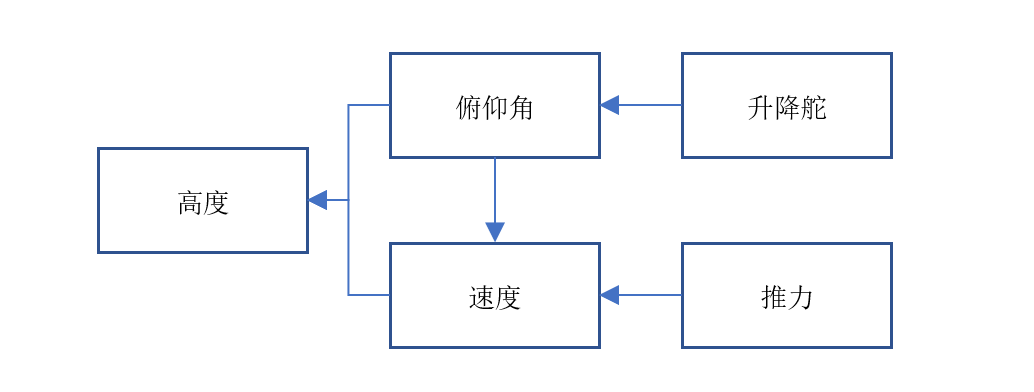
\includegraphics[width=0.75\textwidth]{figures/c3/relation_theta_thrust}
    \caption{速度以及高度通道的控制逻辑图}\label{fig:relation_theta_thrust}
\end{figure}
因而速度和高度需要同时考虑,相应的,期望俯仰角以及推力也需要同时计算。$TECS$控制器正是为此种情况设计的:%TODO:需要添加引用
所谓总能量控制(total energy control)是将无人机的速度以及高度计算得到相应的动能以及势能作为直接控制对象,应用PID控制器对动能与势能的和(total energy)
以及动能与势能的转化(total energy balance)进行控制,计算得到无人机期望俯仰角以及期望推力的控制器。飞机作为一个动力学系统,其机械能来自推力做功的输入,因而总能量控制对应着期望推力;与之对应的俯仰角控制是能量守恒的,
可作为动能向势能(反之亦然)的转化途径,对此种能量转化的控制对应着期望俯仰角。下面简要介绍$TECS$控制器的计算过程:
\\
无人机的总能量为:
\begin{equation}
    E_T=\frac{1}{2}mV_T^2+mgh
    \label{ET}
\end{equation}
对上式两边微分,可得到总能量变化率:
\begin{equation}
    \dot{E_T}=mV_T\dot{V_T}+mg\dot{h}
    \label{ET_rate}
\end{equation}
由此可得单位总能量变化率:
\begin{equation}
    \dot{E}=\frac{\dot{E}_{T}}{m g V_{T}}=\frac{\dot{V}_{T}}{g}+\frac{\dot{h}}{V_{T}}=\frac{\dot{V}_{T}}{g}+\sin \gamma
    \label{specif_ET_rate}
\end{equation}
更换式\ref{point_dynamaic}第一式形式,可得到:
\begin{equation}
    T-D=m g\left(\frac{\dot{V}_{T}}{g}+\sin \gamma\right)
    \label{point_dynamaic_change}
\end{equation}
由此可得:
\begin{equation}
    \Delta T=m g\left(\frac{\dot{V}_{T}}{g}+sin\gamma\right)
    \label{thrust}
\end{equation}
关于能量转化,定义:
\begin{equation}
    B=m g h-\frac{1}{2} m V_{T}^{2}
\end{equation}
能量转化率为:
\begin{equation}
\dot{B}=sin\gamma-\frac{\dot{V}_{T}}{g}
\end{equation}
这里参照开源软件$PX4$内部的TECS控制器设计方法,总能量环和能量分配环的控制逻辑框图如下所示:
\begin{figure}[H]
    \centering
    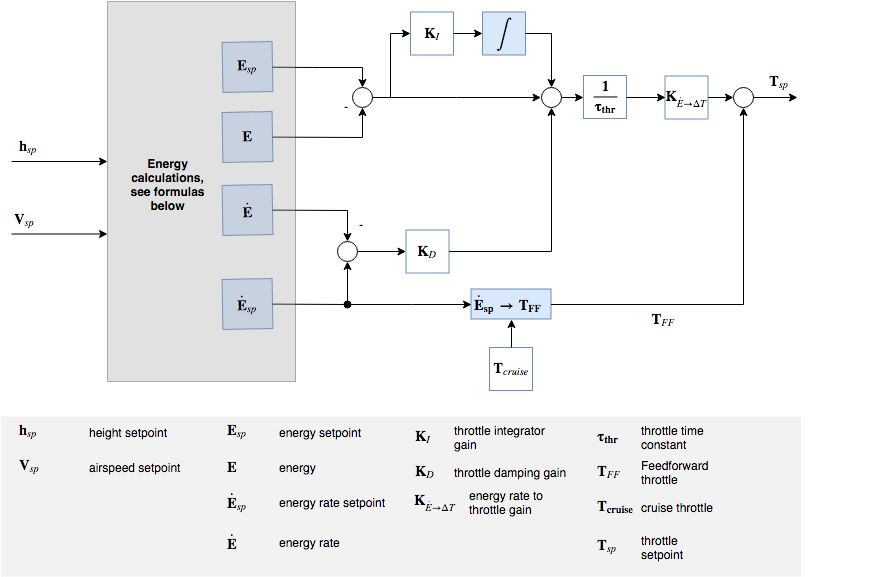
\includegraphics[width=0.75\textwidth]{figures/c3/TECS_throttle.jpg}
    \caption{总能量环}\label{fig:total_energy}
\end{figure}
\begin{figure}[H]
    \centering
    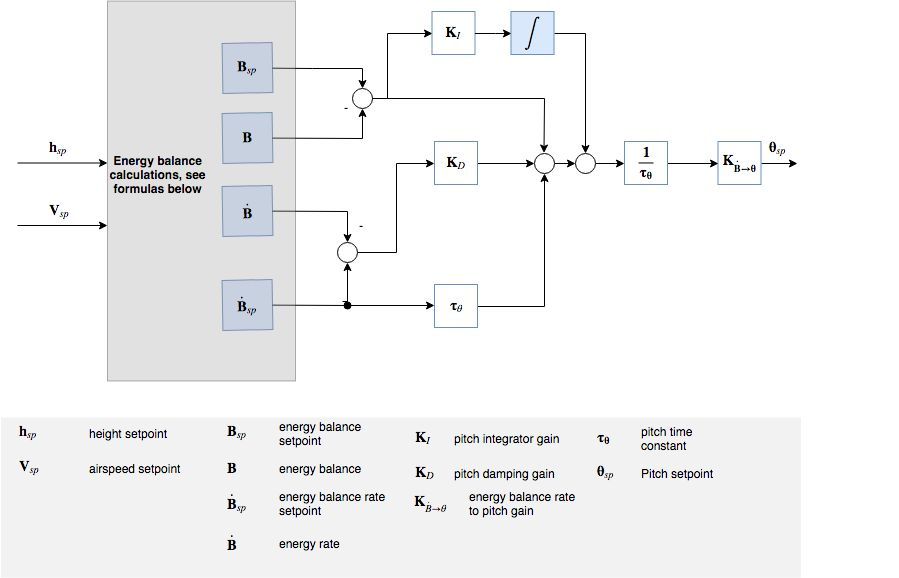
\includegraphics[width=0.75\textwidth]{figures/c3/TECS_pitch.jpg}
    \caption{能量分配环}\label{fig:balance_energy}
\end{figure}
至此,来自水平平面的期望速度$|V|^{des}$以及纵向平面的位置误差$P_{z_b}^{err}$将转化为期望俯仰角以及期望推力进入内环姿态驾驶仪;水平平面编队控制器
产生的期望滚转角也将进入姿态驾驶仪内环。内环姿态自动驾驶仪首先按照无侧滑条件得出期望偏航角速度$\dot{\Phi}^{des}$,然后再利用串级PID分角速度环,角
加速度环计算得到期望的执行机构的偏转角度。但现在的编队控制器还不足以直接用来进行编队控制实现,还需要经过一定的工程处理,详见下一节。
\section{实际应用时的考虑}
在实际应用编队控制器时,按照已有的经验,应主要考虑以下几个方面:
\begin{enumerate}
    \item 在无人机距离期望位置较远以及相对较近时,控制的目的是不完全一致的;应根据不同的控制需求分段设计控制律。
    \item 无人机的空速与地速差距较大(风速很大)时,地速与空速方向不能简单认为一致,应分析之后做相应的处理。
    \item 考虑到无人机各个动力学量的范围,应按照前期对于飞行平台飞行性能计算的结果对控制器计算过程中的各个物理量进行实际限幅。
    \item 离散控制器的频率问题,即内环外环频率关系应当匹配。
    \item 无人机原始信息两量测噪声问题,应设计便于使用的滤波器加以滤波。
\end{enumerate}
相应的,按照上面的问题考虑,有以下解决方案:

\subsection{编队控制器分段设计} 
在位置误差较大时,编队控制器的主要目的应为:以最大速度飞行,迅速减小距离误差。此时无人机速度的期望方向应时刻指向期望点而并非领机的速度方向:
\subsection{风速较大时的处理} 
\subsubsection*{风速因素对于编队控制器的影响分析}
\subsubsection*{风速较大时的改进}
\subsection{无人机飞行性能限幅设计}
按照无人机气动外形尺寸以及基本飞机空气动力学,计算得出的无人机飞行性能如表\ref{tab:flight_performance}所示:
\begin{table}[H]
    \centering
    \caption{无人机飞行性能计算表} \label{tab:flight_performance}
    \begin{tabular*}{0.9\textwidth}{@{\extracolsep{\fill}}c|cccc}
    \toprule
        飞行性能 & $\theta_{max}$ & $\Phi_{max}$ &$V_g^{max}$ & $V_g^{min}$\\
    \midrule
        值 & $\frac{\Pi}{4}$ & $\pm\frac{\Pi}{3}$ & $31.4m/s$ & $8.2m/s$\\
    \bottomrule
\end{tabular*}
\end{table}
\subsection{编队控制器内外环带宽设计}

\subsection{原始数据滤波器设计}
